%!TEX root = ../dissertation.tex

\hypertarget{(chap:inquadramento)}{}
\chapter{Test e validazione}
Una attività di fondamentale importanza è stata quella di testare i modelli e archiviare i dati.
\section{Istanze}
Una \glo{istanza} è un insieme formato dai pacchi da disporre nel contenitore e il contenitore stesso.\\
Un gruppo di istanze è un insieme di istanze diverse tra loro accomunite tra loro dalle dimensioni simili o dal numero di oggetti.\\
Inizialmente ogni qual volta testavamo un modello dopo aver apportato una modifica, eseguivamo un centinaio di test con un gruppo di istanze completamente randomico, l'obiettivo in questo caso era quello di individuare imperfezioni o testare la tenuta dei vincoli.
Successivamente si passava all'esecuzione di 100 test per ciascuna delle istanze riportate di seguito.
\begin{center}
	\begin{tabular}{lrrrr}
		\toprule
		{} & width\_a & width\_b & depth\_a & depth\_b \\
		\midrule
		0  & 0.5      & 2.45     & 0.5      & 2.45     \\
		1  & 0.5      & 1.50     & 0.5      & 4.00     \\
		2  & 1.5      & 2.45     & 0.5      & 4.00     \\
		3  & 0.5      & 1.50     & 3.0      & 4.00     \\
		4  & 1.5      & 2.45     & 3.0      & 4.00     \\
		5  & 0.1      & 1.00     & 0.1      & 1.00     \\
		6  & 0.1      & 1.00     & 3.0      & 4.00     \\
		7  & 2.0      & 2.45     & 3.0      & 4.00     \\
		8  & 2.0      & 2.45     & 2.0      & 2.45     \\
		9  & 0.1      & 1.00     & 0.1      & 4.00     \\
		\bottomrule
	\end{tabular}
	\captionof{table}{Le dimensioni dei gruppi di istanze eseguite}
\end{center}
La tabella riporta gli intervalli entro cui si è deciso randomicamente le dimensioni dei pacchi, ogni gruppo di istanze aveva dimensioni particolari entro cui dovevano trovarsi i pacchi:
\begin{itemize}
	\item \textbf{Larghezza}: [width\_a, width\_b]
	\item \textbf{Profondità}: [depth\_a, depth\_b]
\end{itemize}
\section{Numero di oggetti}
Fin dal modello 2D abbiamo capito che il numero di pacchi per ogni istanza sarebbe stato in numero limitato in quanto dopo 7 pacchi i tempi di esecuzione esplodevano, abbiamo quindi deciso di scegliere in modo randomico in un intervallo [3,10] il numero di pacchi da assegnare a ciascuna istanza, imponendo un \glo{time limit} di 300 secondi, questo portava ad ottenere soluzioni ottime e soluzioni \glo{best bound}, l'analisi dei risultati sarà divisa in queste due categorie infatti.

\begin{figure}[!ht]
	\begin{center} 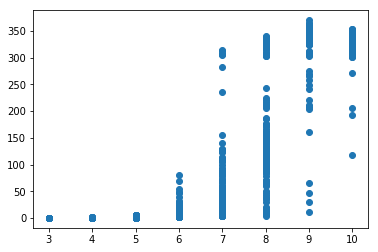
\includegraphics[scale=0.8]{figures/time_nitems}
		\caption[Bin packing figures]{Due contenitori completamente pieni}  
		\label{fig:times}
	\end{center}
\end{figure}

Nel grafico sopra riportato~\eqref{fig:times} viene riportato come ordinata il numero di oggetti e sull'ascissa il tempo espresso in secondi, come si può vedere man mano che gli oggetti aumentano il tempo aumenta notevolmente passando da pochi secondi a minuti, risultano molto interessanti quelle istanze che nonostante abbiano molti oggetti richiedano meno tempo per essere eseguiti, forse questo dovuto alle particolari dimensioni degli oggetti.

\section{Validazione soluzioni fornite}
Di fondamentale importanza per il confronto è stato che le soluzioni fornite dal modello fossero corrette, questo ha richiesto lo sviluppo di alcune funzione che controllassero la validità delle stesse. Per fare questo sono state realizzate le seguenti funzioni:
\begin{itemize}
	\item \textbf{CheckFeasible}: utilizzata per controllare che non vi fossero pacchi che si intersecassero con altri;
	\item \textbf{ChackSequence}: realizzata in due versioni:
	\begin{itemize}
		\item \textbf{2D}: considerando che tutti gli oggetti fossero alla stessa altezza controllava che ciascun pacco avesse almeno una via attraverso cui essere scaricato.
		\item \textbf{3D}: considerava anche la sovrapposizione tra pacchi e oltre a controllare di avere almeno una delle tre direzioni libere rispetto l'altezza a cui si trovava controllava anche se sopra ciascun pacco al momento dello scarico non vi fossero altri pacchi.
	\end{itemize}
	\item \textbf{CheckStable}: utilizzata per controllare la stabilità degli oggetti, questo verificava che l'area di base inferiore poggiasse completamente sulle basi superiori degli oggetti sottostanti;
	\item \textbf{ProjectionCommonArea}: utilizzata per verificare se due parallelepidedi avessero intersezioni tra le loro proiezioni rispetto a 2 assi.
\end{itemize}

Inoltre per natura stessa dei modelli essi restituiscono la soluzione ottima, quindi possiamo dire che se le soluzioni riportate vengono individuate entro il tempo limite e vengono verificate dalle funzioni precedentemente riportate allora queste possono dirsi effettivamente ottime e reali, perfette candidate per un confronto con la soluzione corrispondente fornita dal modello.